% Options for packages loaded elsewhere
\PassOptionsToPackage{unicode}{hyperref}
\PassOptionsToPackage{hyphens}{url}
%
\documentclass[
  ignorenonframetext,
]{beamer}
\usepackage{pgfpages}
\setbeamertemplate{caption}[numbered]
\setbeamertemplate{caption label separator}{: }
\setbeamercolor{caption name}{fg=normal text.fg}
\beamertemplatenavigationsymbolsempty
% Prevent slide breaks in the middle of a paragraph
\widowpenalties 1 10000
\raggedbottom
\setbeamertemplate{part page}{
  \centering
  \begin{beamercolorbox}[sep=16pt,center]{part title}
    \usebeamerfont{part title}\insertpart\par
  \end{beamercolorbox}
}
\setbeamertemplate{section page}{
  \centering
  \begin{beamercolorbox}[sep=12pt,center]{part title}
    \usebeamerfont{section title}\insertsection\par
  \end{beamercolorbox}
}
\setbeamertemplate{subsection page}{
  \centering
  \begin{beamercolorbox}[sep=8pt,center]{part title}
    \usebeamerfont{subsection title}\insertsubsection\par
  \end{beamercolorbox}
}
\AtBeginPart{
  \frame{\partpage}
}
\AtBeginSection{
  \ifbibliography
  \else
    \frame{\sectionpage}
  \fi
}
\AtBeginSubsection{
  \frame{\subsectionpage}
}
\usepackage{amsmath,amssymb}
\usepackage{lmodern}
\usepackage{iftex}
\ifPDFTeX
  \usepackage[T1]{fontenc}
  \usepackage[utf8]{inputenc}
  \usepackage{textcomp} % provide euro and other symbols
\else % if luatex or xetex
  \usepackage{unicode-math}
  \defaultfontfeatures{Scale=MatchLowercase}
  \defaultfontfeatures[\rmfamily]{Ligatures=TeX,Scale=1}
\fi
\usetheme[]{Ilmenau}
% Use upquote if available, for straight quotes in verbatim environments
\IfFileExists{upquote.sty}{\usepackage{upquote}}{}
\IfFileExists{microtype.sty}{% use microtype if available
  \usepackage[]{microtype}
  \UseMicrotypeSet[protrusion]{basicmath} % disable protrusion for tt fonts
}{}
\makeatletter
\@ifundefined{KOMAClassName}{% if non-KOMA class
  \IfFileExists{parskip.sty}{%
    \usepackage{parskip}
  }{% else
    \setlength{\parindent}{0pt}
    \setlength{\parskip}{6pt plus 2pt minus 1pt}}
}{% if KOMA class
  \KOMAoptions{parskip=half}}
\makeatother
\usepackage{xcolor}
\newif\ifbibliography
\setlength{\emergencystretch}{3em} % prevent overfull lines
\providecommand{\tightlist}{%
  \setlength{\itemsep}{0pt}\setlength{\parskip}{0pt}}
\setcounter{secnumdepth}{-\maxdimen} % remove section numbering
\setbeamertemplate{navigation symbols}{}
\setbeamertemplate{footline}[page number]
\usepackage{amsmath}
\ifLuaTeX
  \usepackage{selnolig}  % disable illegal ligatures
\fi
\IfFileExists{bookmark.sty}{\usepackage{bookmark}}{\usepackage{hyperref}}
\IfFileExists{xurl.sty}{\usepackage{xurl}}{} % add URL line breaks if available
\urlstyle{same} % disable monospaced font for URLs
\hypersetup{
  pdftitle={Multivariate Analysis Lecture 6: Sample Covariance Matrix and Wishart Distribution},
  hidelinks,
  pdfcreator={LaTeX via pandoc}}

\title{Multivariate Analysis Lecture 6: Sample Covariance Matrix and
Wishart Distribution}
\author{Zhaoxia Yu\\
Professor, Department of Statistics}
\date{2023-04-20}

\begin{document}
\frame{\titlepage}

\hypertarget{the-big-picture}{%
\section{The Big Picture}\label{the-big-picture}}

\begin{frame}{The Big Picture: Univariate vs Multivariate}
\protect\hypertarget{the-big-picture-univariate-vs-multivariate}{}
\begin{itemize}
\tightlist
\item
  \textcolor{red}{Review}: A random sample, denoted by
  \(X_1, \cdots, X_n\), from a (univariate) normal distribution
  \(N(\mu, \sigma^2)\)

  \begin{itemize}
  \tightlist
  \item
    What are the distributions of \(\bar X, s^2\)? What useful
    statistics can be constructed?
  \end{itemize}
\item
  \textcolor{red}{New material}: A random sample, denoted by
  \(\mathbf X_1, \cdots, \mathbf X_n\), from a multivariate normal
  distribution \(N(\boldsymbol \mu, \boldsymbol \Sigma)\)

  \begin{itemize}
  \tightlist
  \item
    What are the distributions of \(\bar{\mathbf X}, \mathbf S\)? What
    useful statistics can be constructed?
  \end{itemize}
\end{itemize}
\end{frame}

\begin{frame}{The Big Picture: Univariate}
\protect\hypertarget{the-big-picture-univariate}{}
\begin{itemize}
\tightlist
\item
  A random sample, denoted by \(X_1, \cdots, X_n\), from a (univariate)
  normal distribution \(N(\mu, \sigma^2)\)
\item
  Let \(\mathbf X_{n\times 1}=(X_1, \cdots, X_n)^T\). It is random
  vector with a multivarite normal distribution, i.e.,
  \[\mathbf X_{n\times 1}=(X_1, \cdots, X_n)^T \sim \mathbf N(\mu\mathbf 1, \sigma^2\mathbf I)\]
\end{itemize}

\begin{enumerate}
\tightlist
\item
  \(\bar X \sim N(\mu, \sigma^2/n)\)
\item
  \(\frac{(n-1)s^2}{\sigma^2} \sim \chi_{n-1}^2\)
\item
  Independence between \(\bar X\) and \(s^2\).
\item
  a t-statistic is
  \[\frac{\frac{\bar X-\mu}{\sqrt{\sigma^2/n}}}{\sqrt{\frac{(n-1)s^2/\sigma^2}{n-1}}}=\frac{\sqrt{n}(\bar X-\mu)}{s}\]
  It follows the t-distribution with n-1 degrees of freedom, denoted by
  \(t_{n-1}\).
\end{enumerate}
\end{frame}

\begin{frame}{The Big Picture: Multivariate}
\protect\hypertarget{the-big-picture-multivariate}{}
\begin{itemize}
\tightlist
\item
  A random sample \(\mathbf X_1, \cdots, \mathbf X_n\) from a
  multivariate normal distribution
  \(\mathbf N(\boldsymbol \mu, \boldsymbol \Sigma)\).
\item
  Let \[\mathbf X_{n\times p}=\begin{pmatrix}
  \mathbf X_1^T \\ \vdots \\\mathbf X_n^T
  \end{pmatrix}\] \(\mathbf X\) follows a matrix normal distribution.
\end{itemize}

\begin{enumerate}
\item
  Sample mean vector follows a multivariate normal, i.e.,
  \(\bar{\mathbf X} \sim \mathbf N(\boldsymbol \mu, \boldsymbol \Sigma/n)\)
\item
  Sample covariance matrix \((n-1)\mathbf S\) follows a Wishart
  distribution, i.e., \((n-1)\mathbf S \sim Wishart_p (n-1, \Sigma)\)
\item
  Independence between \(\bar {\mathbf X}\) and \(S\).
\item
  Hoetelling's \(T^2\):
  \(T^2 = (\bar{\mathbf X} - \boldsymbol \mu)^T\left(\frac{\mathbf S}{n}\right)^{-1} (\bar{\mathbf X} - \boldsymbol \mu)\)
\end{enumerate}
\end{frame}

\begin{frame}{The Big Picture: outline}
\protect\hypertarget{the-big-picture-outline}{}
\begin{itemize}
\tightlist
\item
  Sample variance and chi-squared distribution
\item
  Sample covariance matrix and Wishart distribution
\item
  Hotelling's \(T^2\)
\item
  Maximum likelihood estimate
\end{itemize}
\end{frame}

\hypertarget{sample-variance}{%
\section{Sample Variance}\label{sample-variance}}

\begin{frame}{Sample Variance and Chi-squared Distribution}
\protect\hypertarget{sample-variance-and-chi-squared-distribution}{}
\begin{itemize}
\tightlist
\item
  Let \(\mathbf X=(X_1, \cdots, X_n)\) denote a random sample from
  \(N(\mu, \sigma^2)\).
\item
  Equivalently, \(\mathbf X \sim N(\mu \mathbf 1, \sigma^2 \mathbf I)\).
\item
  Let \(s^2=\frac{1}{n-1}\sum_{i=1}^n (X_i-\bar X)^2\) denote the sample
  variance.
\item
  We would like to show that
  \[\frac{(n-1)s^2}{\sigma^2}\sim \chi_{n-1}^2\]
\item
  Outline of proof

  \begin{enumerate}
  \tightlist
  \item
    Projection matrices
  \item
    Chi-squared distribution
  \item
    Rewrite \((n-1)s^2/\sigma^2\) as the sum of squared \(N(0,1)\)
    random variables
  \end{enumerate}
\end{itemize}
\end{frame}

\begin{frame}{Projection Matrices}
\protect\hypertarget{projection-matrices}{}
\begin{itemize}
\tightlist
\item
  A projection matrix is a square matrix that is both idempotent and
  symmetric
\end{itemize}

\[\mathbf{P}^2 = \mathbf{P} \mbox{, }\mathbf{P}=\mathbf{P}^T \]
\end{frame}

\begin{frame}{Projection Matrices}
\protect\hypertarget{projection-matrices-1}{}
\begin{itemize}
\tightlist
\item
  Suppose \(\mathbf P\) is a projection matrix. We have

  \begin{itemize}
  \tightlist
  \item
    The eigenvalues of \(\mathbf{P}\) has eigenvalues are either 0 or 1,
    and the number of 1's is the same as the rank of the projection
    matrix.
  \item
    \(tr(\mathbf P) = rank(\mathbf P)\)
  \item
    The spectral decomposition of \(\mathbf P\) is
    \[\mathbf P=\sum_{i=j}^r \gamma_j\gamma_j^T\] where
    \(r=rank(\mathbf P)\), and \((\gamma_1, \cdots, \gamma_r)\) are
    orthogonal vectors of norm 1, i.e.,
  \end{itemize}
\end{itemize}

\[
\gamma_i^T\gamma_j = \left\{
    \begin{array}{ll}
    1 & \mbox{if } i=j\\
    0 & \mbox{if } i\not=j    
    \end{array}
\right.
\]
\end{frame}

\begin{frame}{A Special Projection Matrix: the Centering Matrix}
\protect\hypertarget{a-special-projection-matrix-the-centering-matrix}{}
\begin{itemize}
\tightlist
\item
  The centering matrix
  \(\mathbb C=\mathbf I - \frac{1}{n} \mathbf 1\mathbf 1^T\) is a very
  special matrix.
\item
  It is a projection matrix, which is defined as both symmetric and
  idempotent:

  \begin{itemize}
  \tightlist
  \item
    \(\mathbb C^T=\mathbb C\) (symmetric)
  \item
    \(\mathbb C^2= \mathbb C\) (idempotent)
  \end{itemize}
\item
  One important result about a projection matrix is that its eigenvalues
  are either zero or one.
\item
  By properties of projection matrices, we have

  \begin{itemize}
  \tightlist
  \item
    \(rank(\mathbb C) = tr(\mathbb C)=n-1\)
  \item
    \(\mathbb C = \sum_{j=1}^{n-1}\gamma_j\gamma_j^T\)
  \end{itemize}
\end{itemize}
\end{frame}

\begin{frame}{A Special Projection Matrix: the Centering Matrix}
\protect\hypertarget{a-special-projection-matrix-the-centering-matrix-1}{}
\begin{itemize}
\tightlist
\item
  The centering matrix centers data
\item
  Univariate: Let \(\mathbf X_{n\times 1}\) be a random sample from
  \(N(\mu, \sigma^2)\), i.e.,
  \[\mathbf X_{n\times 1}\sim N(\mu\mathbf 1, \sigma^2 \mathbf I)\]
\end{itemize}

\(\mathbb C\mathbf X\) is a linear function of \(\mathbf X\) and it can
be verified that \(\mathbb C\mathbf 1=\mathbf 0\), we have
\[E[\mathbb C\mathbf X]=\mu \mathbb C\mathbf 1=\mathbf 0\]

\begin{itemize}
\item
  Multivariate: Let \(\mathbf X_{n\times p}\) be a random sample from
  \(N(\boldsymbol\mu, \boldsymbol \Sigma)\) Similarly, it can be shown
  that \(\mathbb C \mathbf X\) has mean \(\mathbf 0_{n\times p}\). We
  have verified this numerically.
\item
  In either situation, we have
  \(\mathbb C \mathbf X = \mathbb C (\mathbf X-E[\mathbf X])\) This fact
  will be used later.
\end{itemize}
\end{frame}

\begin{frame}{Chi-squared distribution}
\protect\hypertarget{chi-squared-distribution}{}
\begin{itemize}
\item
  \textcolor{red}{Definition.} Let \(Z_1, Z_2, ..., Z_k\) be independent
  standard normal random variables. Then, the sum of squares
  \(Q = Z_1^2 + Z_2^2 + ... + Z_k^2\) has a chi-squared distribution
  with \(k\) degrees of freedom, denoted by \(\chi_k^2\).
\item
  Alternative definition. Let
  \(\mathbf Z_{k\times 1} \sim N(\mathbf 0, \mathbf I)\). We say
  \(||\mathbf Z||^2=\mathbf Z^T \mathbf Z\) follows \(\chi_k^2\).
\item
  The PDF of a chi-squared random variable with \(k\) degrees of freedom
  is given by:
\end{itemize}

\[
f(x) = \frac{1}{2^{k/2}\Gamma(k/2)} x^{k/2-1} e^{-x/2} \mbox{,  } x>0
\]

where \(\Gamma(\cdot)\) is the gamma function.
\end{frame}

\begin{frame}{Chi-squared distribution}
\protect\hypertarget{chi-squared-distribution-1}{}
\begin{itemize}
\item
  The chi-squared distribution is a special case of the gamma
  distribution, where the shape parameter is \(k/2\) and the rate
  parameter is 1/2.
\item
  The MGF of a chi-squared random variable with \(k\) degrees of freedom
  is: \[
  M_X(t) = (1-2t)^{-k/2}
  \]
\item
  The mean and variance of a chi-squared random variable with \(k\)
  degrees of freedom are:
\end{itemize}

\[\text{E}[X] = k \mbox{, }\text{Var}[X] = 2k\]
\end{frame}

\begin{frame}{Construct Chi-squared R.V.s using Normal R.V.s and
Projection Matrices}
\protect\hypertarget{construct-chi-squared-r.v.s-using-normal-r.v.s-and-projection-matrices}{}
\begin{itemize}
\tightlist
\item
  Let \(\mathbf P_{n\times n}\) be a projection matrix with rank \(r\)
  and let \(\mathbf Z_{n\times 1}\sim N(\mathbf 0, \mathbf I)\) \[
  \begin{aligned}
  \mathbf Z^T \mathbf P \mathbf Z &= \mathbf Z^T \sum_{i=1}^r \gamma_i \gamma_i^T \mathbf Z= \sum_{i=1}^r \mathbf Z^T \gamma_i \gamma_i^T \mathbf Z\\
  &= \sum_{i=1}^r (\gamma_i^T \mathbf Z)^T(\gamma_i^T \mathbf Z)
  \end{aligned}
  \]
\end{itemize}

Let \(Y_i = \gamma_i^T \mathbf Z\). Note that \(Y_i\) is univariate and
it is a linear combination of \(\mathbf Z\), from which we can show that
\(Y_i \sim N(0, 1)\).

\begin{itemize}
\tightlist
\item
  Note that \(\mathbf Z^T \mathbf P \mathbf Z=\sum_{i=1}^r Y_i^2\). By
  the definition of chi-squared distribution, we have
  \(\mathbf Z^T \mathbf P \mathbf Z\sim \chi_r^2\)
\end{itemize}
\end{frame}

\begin{frame}{The Sample Variance}
\protect\hypertarget{the-sample-variance}{}
\begin{itemize}
\tightlist
\item
  We have shown that

  \begin{itemize}
  \tightlist
  \item
    \(\mathbb C = \mathbf I - \frac{1}{n} \mathbf 1 \mathbf 1^T\)
  \item
    \(\mathbb C^T=\mathbb C\), \(\mathbb C^2=\mathbb C\).
  \item
    It is a projection matrix with rank \(n-1\) and
    \[\mathbb C = \sum_{j=1}^{n-1}\gamma_i\gamma_i^T\] -The he centering
    matrix does center data, i.e.,
    \[\mathbb C \mathbf X = \mathbb C (\mathbf X - E[\mathbf X])\]
  \item
    \((n-1)s^2=\mathbf X^T\mathbb C \mathbf X\), where
  \end{itemize}
\end{itemize}
\end{frame}

\begin{frame}{The Sample Variance}
\protect\hypertarget{the-sample-variance-1}{}
\begin{itemize}
\tightlist
\item
  Therefore, \[
  \begin{aligned}
  \frac{(n-1)s^2}{\sigma^2}&=\frac{(\mathbf X - E[\mathbf X])^T}{\sigma}\mathbb C^T \mathbb C \mathbb C \frac{(\mathbf X - E[\mathbf X])}{\sigma}\\
  &=\frac{(\mathbf X - E[\mathbf X])^T}{\sigma}\mathbb C \frac{(\mathbf X - E[\mathbf X])}{\sigma}
  \end{aligned}\]
\end{itemize}
\end{frame}

\begin{frame}{The Sample Variance}
\protect\hypertarget{the-sample-variance-2}{}
\begin{itemize}
\tightlist
\item
  Let \[\mathbf Z=\frac{(\mathbf X - E[\mathbf X])}{\sigma}\]
\item
  Easy to see that \(\mathbf Z\sim N(\mathbf 0, \mathbf I)\). Thus,
\end{itemize}

\[\frac{(n-1)s^2}{\sigma^2}=\mathbf Z^T \mathbb C \mathbf Z\]

\begin{itemize}
\tightlist
\item
  Use the result in previous slides, we have
  \[\frac{(n-1)s^2}{\sigma^2}=\mathbf Z^T \mathbb C \mathbf Z \sim \chi_{n-1}^2\]
\end{itemize}
\end{frame}

\hypertarget{sample-covariance}{%
\section{Sample Covariance}\label{sample-covariance}}

\begin{frame}{The Sample Covriance from A MVN Random Sample}
\protect\hypertarget{the-sample-covriance-from-a-mvn-random-sample}{}
\begin{itemize}
\tightlist
\item
  Let
  \(\mathbf X_1, \cdots,\mathbf X_n \overset{iid} \sim N(\boldsymbol \mu, \boldsymbol \Sigma)\).
\item
  Recall that the sample covariance matrix is defined as
  \[\mathbf S =\frac{1}{n-1} \sum_{i=1}^n (\mathbf X_i - \bar{\mathbf X})(\mathbf X_i - \bar{\mathbf X})^T\]
\item
  We have shown that
  \[(n-1)\mathbf S = \mathbf X ^T \mathbb C \mathbf X\] where
  \(\mathbf X\) is the \(n\times p\) random matrix.
\end{itemize}
\end{frame}

\begin{frame}{The Sample Covriance from A MVN Random Sample}
\protect\hypertarget{the-sample-covriance-from-a-mvn-random-sample-1}{}
\begin{itemize}
\tightlist
\item
  The goal is to show that \((n-1)\mathbf S\) follows a Wishart
  distribution. More specifically, we would like to show that
  \[(n-1)\mathbf S \sim Wishart_p(n-1, \Sigma)\]
\item
  Outline of proof

  \begin{enumerate}
  \tightlist
  \item
    Wishart-distribution
  \item
    Rewrite \((n-1)\mathbf S\)
  \item
    Apply properties of a projection matrix
  \item
    Use the definition of Wishart distribution
  \end{enumerate}
\end{itemize}
\end{frame}

\begin{frame}{Wishart Distribution}
\protect\hypertarget{wishart-distribution}{}
\begin{itemize}
\item
  The Wishart distribution is named after the British statistician John
  Wishart, who introduced it in his 1928 paper published in Biometrika.
\item
  Wishart was interested in the problem of estimating the covariance
  matrix of a multivariate normal distribution.
\item
  Wishart showed that the sample covariance matrix follows a particular
  probability distribution that we now call the Wishart distribution.
\item
  The Wishart distribution has become a fundamental tool in multivariate
  statistical analysis
\end{itemize}
\end{frame}

\begin{frame}{Definition of Wishart Distribution}
\protect\hypertarget{definition-of-wishart-distribution}{}
\begin{itemize}
\item
  A Wishart distribution can be defined in the following way
\item
  Let \(\mathbf W\) be a \(p\times p\) random matrix. We say
  \(\mathbf W\) follows \(Wishart_{p}(k, \boldsymbol \Sigma)\) if
  \(\mathbf W\) can be written as \(\mathbf W=\mathbf X^T \mathbf X\)
  where \(\mathbf X\) denotes the random matrix formed by a random
  sample of size \(k\) from MVN \(N(\mathbf 0, \boldsymbol \Sigma)\).
\item
  The definition indicates that if we have a random sample
  \(\mathbf X_1, \cdots \mathbf X_k\) from
  \(N(\mathbf 0, \boldsymbol \Sigma)\), then
  \(\mathbf X^T \mathbf X=\sum_{i=1}^k \mathbf X_i \mathbf X_i^T \sim Wishart_p(k, \boldsymbol \Sigma)\).
\item
  Remark:\(E[\mathbf W]=k\Sigma\).
\end{itemize}
\end{frame}

\begin{frame}{Wishart vs Chi-squared}
\protect\hypertarget{wishart-vs-chi-squared}{}
\begin{itemize}
\item
  \textcolor{red}{Wishart}: If
  \(\mathbf X_1, \cdots \mathbf X_k \overset{iid}\sim N(\mathbf 0, \boldsymbol \Sigma)\),
  then
  \[\mathbf X^T \mathbf X =\sum_{i=1}^k \mathbf X_i\mathbf X_i^T \sim Wishart_p(k, \boldsymbol \Sigma) \mbox{, where } \mathbf X_{k\times p}=\begin{pmatrix}
  X_1^T\\ \vdots\\ X_k^T
  \end{pmatrix}
  \]
\item
  \textcolor{red}{Chi-squared}: If
  \(X_1, \cdots, X_k \overset{iid}\sim N(0,1)\), then\\
  \[\mathbf X^T\mathbf X=\sum_{i=1}^k X_i^2\sim \chi_k^2 \mbox{, where } \mathbf X_{k\times 1}= 
  \begin{pmatrix}
  X_1 \\ \vdots \\ X_k
  \end{pmatrix}\]
\end{itemize}
\end{frame}

\begin{frame}{Wishart vs Chi-squared (continued)}
\protect\hypertarget{wishart-vs-chi-squared-continued}{}
\begin{itemize}
\tightlist
\item
  When \(p=1\),
  \[W=\sum_{i=1}^k X_i^2 = \sigma^2 \sum_{i=1}^k \left(\frac{X_i}{\sigma} \right)^2\sim \sigma^2 \chi_k^2 \]
\end{itemize}
\end{frame}

\begin{frame}{The Sample Covariance Matrix}
\protect\hypertarget{the-sample-covariance-matrix}{}
\begin{itemize}
\item
  Let \(\mathbf X_1, \cdots \mathbf X_n\) be a random sample from
  \(N(\boldsymbol \mu, \boldsymbol \Sigma)\). The
  \(\mathbf X_{n\times p}\) follows a matrix normal distribution:
  \[\mathbf X \sim N(\mathbf 1_n \otimes \boldsymbol \mu^T, \boldsymbol \Sigma, \mathbf I_n)\]
\item
  The sample covariance
  \((n-1)\mathbf S=\mathbf X^T \mathbb C \mathbf X\) is based on the
  centered data. The definition of Wishart distribution is not
  applicable immediately.
\item
  Next we show that \((n-1)\mathbf S\) follows
  \(Wishart_p(n-1, \boldsymbol\Sigma)\).
\end{itemize}
\end{frame}

\begin{frame}{The Sample Covariance Matrix}
\protect\hypertarget{the-sample-covariance-matrix-1}{}
\begin{itemize}
\tightlist
\item
  Rewrite \((n-1)\mathbf S\): \[
  \begin{aligned}
  (n-1)\mathbf S&=\mathbf X^T \mathbb C^T\mathbb C\mathbb C \mathbf X=(\mathbb C \mathbf X)^T(\mathbb C \mathbf X)\\
  &=(\mathbb C \mathbf X)^T\mathbb C(\mathbb C \mathbf X)\\
  &=(\mathbb C \mathbf X)^T\sum_{j=1}^{n-1}\gamma_i \gamma_i^T (\mathbb C \mathbf X)\\
  &=\sum_{j=1}^{n-1} (\gamma_i^T \mathbb C \mathbf X)^T (\gamma_i^T \mathbb C \mathbf X)
  \end{aligned}\]
\end{itemize}
\end{frame}

\begin{frame}{The Sample Covariance Matrix}
\protect\hypertarget{the-sample-covariance-matrix-2}{}
\begin{itemize}
\tightlist
\item
  Let \(Y_i= (\gamma_i^T \mathbb C \mathbf X)^T\), we have

  \begin{itemize}
  \tightlist
  \item
    \(E[Y_i]=0\) because \(\mathbb C\) is the centering matrix
  \item
    In the following, we show that \(Y_i\) and \(Y_j\) are uncorrelated
    for \(i\not=j\):
  \end{itemize}
\end{itemize}

\[\begin{aligned}
  Cov[Y_i, Y_j]&=E[(Y_i-\mathbf 0 )(Y_j-\mathbf 0)^T]\\
  &= E[Y_iY_j^T] \\
  &= E[(\gamma_i^T \mathbb C \mathbf X)^T(\gamma_j^T \mathbb C \mathbf X)]\\
  &= E[\mathbf X^T \mathbb C \gamma_i \gamma_j^T \mathbb C \mathbf X] \\
  &=\mathbf 0
  \end{aligned}\]

The last step is true because for \(i\not=j\), \(\gamma_i \gamma_j^T=0\)
\end{frame}

\begin{frame}{The Sample Covariance Matrix}
\protect\hypertarget{the-sample-covariance-matrix-3}{}
Since \(Y_i\) and \(Y_j\) are two linear combinations of the same MVN
distributed random matrix (or its vectorized version), we have \(Y_i\)
and \(Y_j\) are independent for \(i\not=j\).

\begin{itemize}
\item
  It can also be shown that \(Y_i \sim N(\mathbf 0, \Sigma)\).
\item
  By the definition of Wishart, we can conclude that
  \[(n-1)\mathbf S\sim Wishart_p(n-1, \boldsymbol \Sigma)\]
\end{itemize}
\end{frame}

\begin{frame}{Some Interesting Results}
\protect\hypertarget{some-interesting-results}{}
\begin{itemize}
\item
  Consider a random sample from MVN
  \(N(\boldsymbol \mu, \boldsymbol \Sigma)\). Let \(\mathbf S\) denote
  the sample covariance matrix.
\item
  We have already shown that
  \((n-1)\mathbf S \sim Wishart_p(n-1, \boldsymbol \Sigma)\)
\item
  What is the distribution of a diagonal element of \((n-1)\mathbf S\)?
\item
  What is the distribution of the sum of elements of \((n-1)\mathbf S\)?
\item
  What is the distribution of \((n-1)\mathbf B \mathbf S \mathbf B^T\)
  where \(B\) is a fixed \(q\times p\) matrix?
\item
  If time permits, we will run some simulations
\end{itemize}
\end{frame}

\begin{frame}{Some Interesting Results (continued)}
\protect\hypertarget{some-interesting-results-continued}{}
\begin{itemize}
\item
  If you cannot get the answer to the last question, let's use the
  definition of Wishart distribution.
\item
  Let \(\mathbf W = (n-1)S\). Because it follows
  \(Wishart_p(n-1, \boldsymbol\Sigma)\), we know that
  \(\mathbf W=\sum_{j=1}^{n-1} \mathbf Z_j \mathbf Z_j^T\) where
  \(\mathbf Z_j\)'s are iid frm \(N(\mathbf 0, \boldsymbol\Sigma)\).
\item
  Then \[
  \begin{aligned}
  (n-1)\mathbf B \mathbf S \mathbf B^T &= \mathbf B\sum_{j=1}^{n-1} \mathbf Z_j \mathbf Z_j^T\mathbf B = \sum_{j=1}^{n-1} \mathbf B \mathbf Z_j \mathbf Z_j^T\mathbf B^T\\
  &= \sum_{j=1}^{n-1} (\mathbf B \mathbf Z_j)(\mathbf B \mathbf Z_j)^T
  \end{aligned}
  \]
\end{itemize}
\end{frame}

\begin{frame}{Some Interesting Results (continued)}
\protect\hypertarget{some-interesting-results-continued-1}{}
Let \(\mathbf Y_j=\mathbf B \mathbf Z_j\). Note that it is a linear
function of \(\mathbf Z_j\); therefore
\[\mathbf Y_j\sim N(\mathbf 0, \mathbf B \boldsymbol \Sigma \mathbf B^T)\]
and the \(\mathbf Y_j\)'s are iid (becaue \ldots).

By the definition of Wishart distribution, we have

\[(n-1)\mathbf B \mathbf S \mathbf B^T\sim Wishart_q(n-1, \mathbf B \boldsymbol \Sigma \mathbf B^T)\]
\end{frame}

\hypertarget{hotellings-t2}{%
\section{\texorpdfstring{Hotelling's
\(T^2\)}{Hotelling's T\^{}2}}\label{hotellings-t2}}

\begin{frame}{The Hotelling's \(T^2\) Statistic}
\protect\hypertarget{the-hotellings-t2-statistic}{}
\begin{itemize}
\item
  Finally we are ready to introduce Hotelling's
\item
  The student's t is used for making inference of mean(s) of normal
  distribution(s)
\item
  Hotelling generalized the student's t, which is for univarite, to
  Hotelling's T2, which the multivariate version
\end{itemize}
\end{frame}

\begin{frame}{Definition Hotelling's \(T^2\)}
\protect\hypertarget{definition-hotellings-t2}{}
\begin{itemize}
\tightlist
\item
  \textcolor{red}{Definition. }We say a random variable follows
  Hotelling's \(T^2\) \(T_{p,\nu}^2\) if the random variable can be
  written as \(\mathbf Z^T\left(\frac{W}{\nu}\right)^{-1}\mathbf Z\)
  where

  \begin{enumerate}
  \tightlist
  \item
    \(\mathbf Z\sim N(\mathbf 0, \boldsymbol\Sigma)\)
  \item
    \(\mathbf W \sim W_p(\nu, \boldsymbol\sigma)\)
  \item
    \(\mathbf Z \perp \mathbf W\)
  \end{enumerate}
\end{itemize}
\end{frame}

\begin{frame}{One-Sample Hotelling \(T^2\)}
\protect\hypertarget{one-sample-hotelling-t2}{}
\begin{itemize}
\tightlist
\item
  Let \(\boldsymbol{X}_1, \boldsymbol{X}_2, ..., \boldsymbol{X}_n\) be a
  random sample from a multivariate normal distribution with mean vector
  \(\boldsymbol{\mu}\) and covariance matrix \(\boldsymbol{\Sigma}\).
\item
  The sample mean vector and sample covariance matrix are denoted by
  \(\bar{\mathbf X}\) and \(\mathbf S\), respectively.
\item
  The null hypothesis of interest
  \(H_0: \boldsymbol \mu = \boldsymbol \mu_0\)
\item
  The one-sample Hotelling \(T^2\) is defined as
  \[T^2=(\hat{\mathbf \mu} - \mathbf \mu_0)^T \left(Cov(\hat{\mathbf \mu})\right)^{-1}(\hat{\mathbf \mu} - \mathbf \mu_0)\]
\end{itemize}
\end{frame}

\begin{frame}{One-Sample Hotelling \(T^2\) (continued)}
\protect\hypertarget{one-sample-hotelling-t2-continued}{}
\begin{itemize}
\item
  To see that \(T^2\) does follow Hotelling's \(T^2\), we rewrite it \[
  \begin{aligned}
  T^2&=(\hat{\mathbf \mu} - \mathbf \mu_0)^T \left(Cov(\hat{\mathbf \mu})\right)^{-1}(\hat{\mathbf \mu} - \mathbf \mu_0)\\
  &= (\bar{\mathbf X} - \mathbf \mu_0)^T \left(Cov(\bar{\mathbf X})\right)^{-1}(\bar{\mathbf X} - \mathbf \mu_0)\\
  &= (\bar{\mathbf X} - \mathbf \mu_0)^T \left(\frac{S}{n}\right)^{-1}(\bar{\mathbf X} - \mathbf \mu_0)\\
  &= [\sqrt{n}(\bar{\mathbf X} - \mathbf \mu_0)]^T \left(\frac{(n-1)S}{n-1}\right)^{-1}[\sqrt{n}(\bar{\mathbf X} - \mathbf \mu_0)]
  \end{aligned}
  \]
\item
  We have shown that all the three conditions for constructing a
  Hotelling's \(T^2\) are satisfied
\item
  As a result, \(T^2\sim T_{p, n-1}^2\).
\end{itemize}
\end{frame}

\begin{frame}{Hotelling's \(T^2\) Distribution vs \(F\) Distribution}
\protect\hypertarget{hotellings-t2-distribution-vs-f-distribution}{}
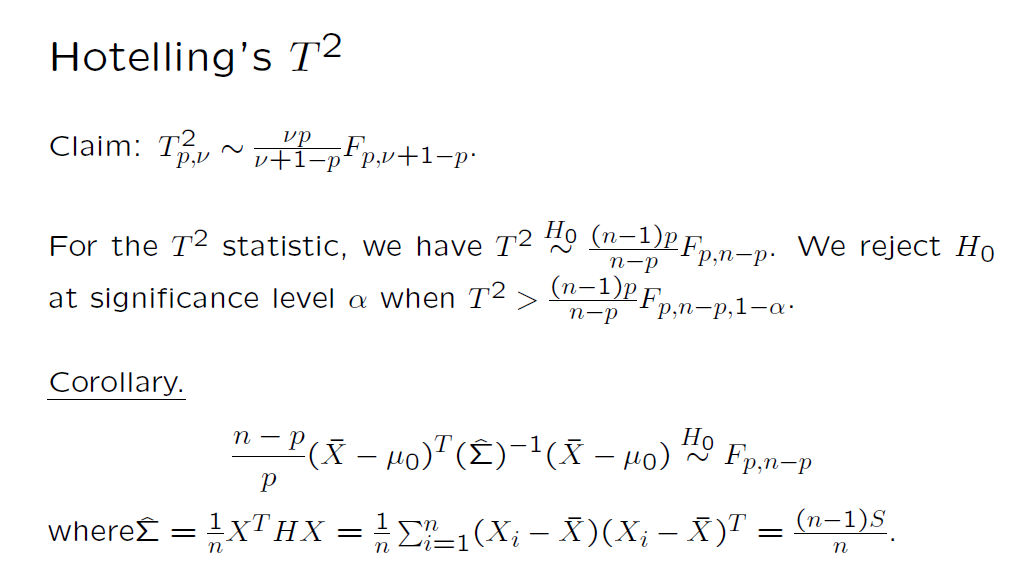
\includegraphics[width=0.8\linewidth]{img/T2vsF}
\end{frame}

\hypertarget{mle}{%
\section{MLE}\label{mle}}

\begin{frame}{MLE: Introduction}
\protect\hypertarget{mle-introduction}{}
\begin{itemize}
\item
  The maximum likelihood estimate (MLE) is a widely used method for
  estimating the parameters of a statistical model.
\item
  In this presentation, we will focus on the MLE for a multivariate
  normal distribution.
\end{itemize}
\end{frame}

\begin{frame}{MLE: Multivariate Normal Distribution}
\protect\hypertarget{mle-multivariate-normal-distribution}{}
\begin{itemize}
\tightlist
\item
  A random vector \(\boldsymbol{X}\) follows a \(p\)-dimensional
  multivariate normal distribution with mean vector \(\boldsymbol{\mu}\)
  and covariance matrix \(\boldsymbol{\Sigma}\), denoted by
  \(\boldsymbol{X} \sim \mathcal{N}_p(\boldsymbol{\mu}, \boldsymbol{\Sigma})\),
  if its probability density function is given by:
\end{itemize}

\[
f_{\boldsymbol{X}}(\boldsymbol{x}) = \frac{1}{(2\pi)^{p/2} |\boldsymbol{\Sigma}|^{1/2}} \exp\left(-\frac{1}{2} (\boldsymbol{x} - \boldsymbol{\mu})^T \boldsymbol{\Sigma}^{-1} (\boldsymbol{x} - \boldsymbol{\mu})\right)
\]

where \(|\boldsymbol{\Sigma}|\) denotes the determinant of
\(\boldsymbol{\Sigma}\).
\end{frame}

\begin{frame}{MLE:Maximum Likelihood Estimate}
\protect\hypertarget{mlemaximum-likelihood-estimate}{}
\begin{itemize}
\item
  Let \(\boldsymbol{X}_1, \boldsymbol{X}_2, ..., \boldsymbol{X}_n\) be a
  random sample from a multivariate normal distribution with mean vector
  \(\boldsymbol{\mu}\) and covariance matrix \(\boldsymbol{\Sigma}\).
\item
  The log-likelihood function for the sample is given by:
\end{itemize}

\[
\ell(\boldsymbol{\mu}, \boldsymbol{\Sigma}) = -\frac{n}{2} \log(2\pi) -\frac{n}{2} \log|\boldsymbol{\Sigma}| - \frac{1}{2} \sum_{i=1}^n (\boldsymbol{X}_i - \boldsymbol{\mu})^T \boldsymbol{\Sigma}^{-1} (\boldsymbol{X}_i - \boldsymbol{\mu})
\]

\begin{itemize}
\tightlist
\item
  The MLE of \(\boldsymbol{\mu}\) is the sample mean
  \(\bar{\boldsymbol{X}} = \frac{1}{n} \sum_{i=1}^n \boldsymbol{X}_i\).
\end{itemize}
\end{frame}

\begin{frame}{MLE:Maximum Likelihood Estimate (continued)}
\protect\hypertarget{mlemaximum-likelihood-estimate-continued}{}
\begin{itemize}
\tightlist
\item
  To derive the MLE of \(\boldsymbol{\Sigma}\), we first take the
  derivative of the log-likelihood function with respect to
  \(\boldsymbol{\Sigma}\) and set it equal to zero:
\end{itemize}

\[
\frac{\partial \ell}{\partial \boldsymbol{\Sigma}} = -\frac{n}{2} \boldsymbol{\Sigma}^{-1} + \frac{1}{2} \sum_{i=1}^n (\boldsymbol{X}_i - \boldsymbol{\mu})(\boldsymbol{X}_i - \boldsymbol{\mu})^T \boldsymbol{\Sigma}^{-2} = 0
\]

\begin{itemize}
\tightlist
\item
  Solving for \(\boldsymbol{\Sigma}\), we obtain the MLE as:
\end{itemize}

\[
\boldsymbol{\hat{\Sigma}} = \frac{1}{n} \sum_{i=1}^n (\boldsymbol{X}_i - \boldsymbol{\hat{\mu}})(\boldsymbol{X}_i - \boldsymbol{\hat{\mu}})^T
\]

\begin{itemize}
\tightlist
\item
  where \(\boldsymbol{\hat{\mu}}\) is the MLE of \(\boldsymbol{\mu}\),
  as previously derived.
\end{itemize}
\end{frame}

\end{document}
